\chapter{机械能}\label{chapter-mechanical-energy}

\section{功}
功这个概念是十九世纪当人们广泛使用各种机械时在力学中出现的.从人的劳动到各种机械的工作,人们发现它们有一个共同的特点:有力作用在物体上,而且物体在力的作用下发生一段位移.引入功的概念,就是为了反映这个共同的特点.一个物体受到力的作用,如果在力的方向上发生一段位移,物理学中就说这个力对物体做了功.人推车前进,车在人的推力下发生一段位移,推力对车做了功.起重机提起货物,货物在起重机钢绳的拉力下发生一段位移,拉力对货物做了功.机车牵引列车前进,列车在机车的牵引力下发生位移,牵引力对列车做了功.

如果有力作用在物体上,而物体没有在这个力的方向发生位移,这个力对物体就没有做功.一个人举着一个物体不动,他虽然对这个物体作用一个向上的支持力,但这个支持力对物体并没有做功.人用力推一个笨重的物体而没有推动,他虽然对这个物体作用一个向前的推力,这个推力也没有对物体做功.人在水平面上推车前进,重力并没有对车做功,因为重力的方向是竖直向下的,车虽然发生了位移,但在重力的方向上却没有位移.功这个概念和一般所说的“做工”或“工作”
含意不同.在物理学中,\NoteUnderWave{力和物体在力的方向上发生的位移,是做功的两个不可缺少的因素}.

\subsection{功的公式}

功的大小是由力的大小和物体在力的方向上发生的位移的大小确定的.力越大,位移越大,功就越大.我们在初中学过,如果力的方向跟物体运动的方向一致(图~\ref{fig_A_7-1}),功就等于力的大小和位移的大小的乘积.
用$F$表示力的大小,用$s$表示位移的大小,用$W$表示力所做的功,那么,
\[W=Fs\]

\begin{figure}[htbp]
    \centering
    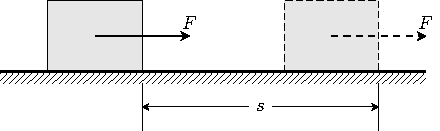
\includegraphics{fig/A/7-1.pdf}
    \caption{}\label{fig_A_7-1}
\end{figure}

但是,物体运动的方向不一定总跟力的方向一致,当力的方向跟运动方向成某一角度$\alpha$时(图~\ref{fig_A_7-2}),怎样来计算这个力所做的功呢?我们可以把力$F$分解成两个分力:跟位移方向一致的分力$F_1$,跟位移方向垂直的分力$F_2$.设物体在力$F$作用下发生的位移的大小是$s$,力$F_1$所做的功等于$F_1s$.
力$F_2$的方向跟位移的方向垂直,在$F_2$的方向上没有发生位移,力$F_2$所做的功等于零.因此,力$F$对物体所做的功就等于$F_1s$,而$F_1=F\cos\alpha$,所以
\[W=Fs\cos\alpha \]

\begin{figure}[htbp]
    \centering
    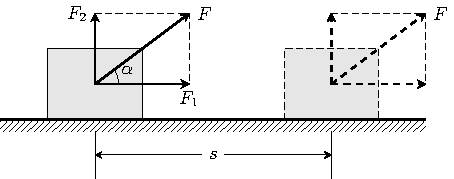
\includegraphics{fig/A/7-2.pdf}
    \caption{}\label{fig_A_7-2}
\end{figure}

这就是说,\NoteUnderWave{力对物体所做的功,等于力的大小、位移的大小、力和位移的夹角的余弦三者的乘积}.

这个公式是计算功的一般的公式.
当$\alpha=0$时,$\cos\alpha=1$,$W=Fs$,这就是初中学过的公式.当$\alpha=\pi/2$时,$\cos\alpha=0$,$W=0$,表示力的方向与位移方向垂直时,力不做功.

功是由力的大小和位移的大小确定的,它没有方向,是一个标量.
在国际单位制中,功的单位是\NoteBold{焦耳},简称焦,国际符号是$\UJA$.
1焦就是1牛的力使物体在力的方向上发生1米位移所做的功.
\[1 \UJ=1 \UN \times 1 \Um=1 \UNm \]

\subsection{正功和负功} 

现在我们讨论一下功的公式$W=Fs\cos\alpha$.如果力的方向与位移的方向之间的夹角小于90$^\circ$,即$\alpha<\pi/2$,那么
$\cos\alpha>0$,$W>0$,即力对物体做正功.人推车前进的时候,$\alpha<\pi/2$,人的推力对车做正功.
物体在重力作用下下落的时候,$\alpha=0$,重力对物体做正功(图~\ref{fig_A_7-3}).
\begin{figure}[htbp]
    \centering
    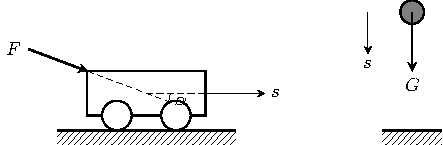
\includegraphics{fig/A/7-3.pdf}
    \caption{动力对物体做正功}\label{fig_A_7-3}
\end{figure}

如果力的方向与位移的方向之间的夹角大于90$^\circ$而小于或等于180$^\circ$,即$\pi/2<\alpha\le \pi$,那么$\cos\alpha <0$,$W<0$,即力对物体做负功.人用力阻碍车前进的时候,$\pi/2<\alpha\le \pi$,人的推力对车做负功.
前进的车在摩擦力作用下逐渐停下来,$\alpha=\pi$,$\cos\alpha=-1$,摩擦力对车做负功.上抛物体在向上运动的时候,$\alpha=\pi$,$\cos\alpha=-1$,重力对物体做负功(图~\ref{fig_A_7-4}).
\begin{figure}[htbp]
    \centering
    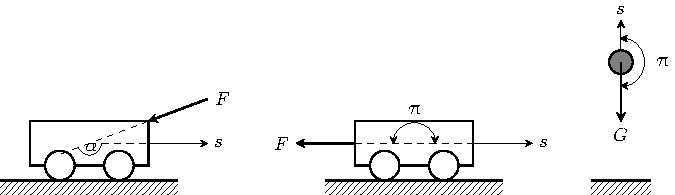
\includegraphics{fig/A/7-4.pdf}
    \caption{阻力对物体做负功}\label{fig_A_7-4}
\end{figure}

一个力对物体做了负功,往往也说成物体克服这个力做
了功(取正值).比如一个力对物体做了$-6$焦耳的功,也可以说物体克服这个力做了6焦耳的功.上抛物体向上运动时重力对物体做负功,也可以说物体克服重力做了功.汽车在关闭发动机以后,在阻力作用下停下来,阻力做负功,也可以说汽车克服阻力做了功.

\subsection*{练习一}
\begin{enumerate}
    \item 在起重机的钢绳上挂着重物,当重物静止时,钢绳的拉力有没有做功?重力有没有做功?

    在水平桌面上滚动的小球,桌面对球的支持力有没有做功?重力有没有做功?
    \item 在厘米$\cdot$克$\cdot$秒制中,功的单位叫做\NoteBold{尔格}($\UergA$).1尔格是1达因($\Udyn$)的力使物体在力的方向上发生1厘米的位移所做的功.
    试证明:
    \[1 \UJ=10^7 \Uerg \]
    \item 在水平道路上匀速前进的汽车受到哪些力的作用?其中哪些力做功,哪些力没有做功?哪个力做正功,哪个力做负功?
    \item 在图~\ref{fig_A_7-5a} 中,力$F$是350牛,在这个力的作用下,物体加速向右移动了1.5米,力$F$所做的功是多少?在图~\ref{fig_A_7-5b} 中,力$F$是250牛,在这个力的作用下,物体减速向右移动了2.5米,力$F$所做的功是多少?

\begin{figure}[htbp]
    \centering
    \begin{subfigure} {0.4\linewidth} 
        \centering
        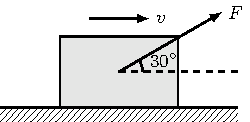
\includegraphics{fig/A/7-5a.pdf} 
        \caption{}\label{fig_A_7-5a} 
    \end{subfigure}
    \hfil
    \begin{subfigure} {0.4\linewidth} 
        \centering
        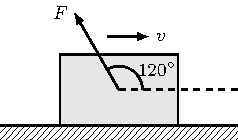
\includegraphics{fig/A/7-5b.pdf} 
        \caption{}\label{fig_A_7-5b} 
    \end{subfigure}
    \caption{}\label{fig_A_7-5}
\end{figure}

    \item 用起重机把重物从地面匀速地提到5米高的地方,重物的重量是$2\times 10^4$牛,钢绳的拉力做多少功?重力做多少功?重物克服重力所做的功是多少?
    \item 一只装货的木箱,质量是35千克,木箱和地面之间的摩擦系数是0.2.沿水平方向用力推木箱,使它在水平地面上匀速移动8.0米,推力所做的功是多少?木箱克服摩擦力所做的功是多少?
    \item 一个物体,重量是10牛,在水平拉力的作用下,一次在光滑水平面上移动了0.5米的距离,另一次在粗糙水平面上移动了相同的距离.粗糙面和物体间的滑动摩擦系数是0.2.两次所受的拉力都是15牛.在这两种情况下,拉力所做的功是否相同?
\end{enumerate}

\section{功率}

不同物体做相同的功,所用的时间往往并不一样,也就是
说,做功的快慢并不相同.一台起重机在10分钟内可以把1吨重的货物举高到预定的高度,而另一台只用30秒就可以做相同的功,第二台就比第一台做功快19倍.

在物理学上用功率表示做功的快慢.
\NoteUnderWave{功跟完成这些功所用时间的比值,叫做功率}.如果用$P$表示功率,$W$表示功,$t$表示时间,那么,
\[P=\frac{W}{t}\]

在国际单位制中,功率的单位是瓦特,简称瓦,国际符号是$\UWA$.
$1 \UW = 1 \UJs$.
%1瓦=1焦/秒.
瓦特这个单位比较小,技术上常用千瓦($\UkWA$)和马力($\UHPA$) %Horsepower
做功率的单位.
\[1 \UkW=1000\UW,\qquad 1 \UHP \approx 0.735 \UkW \]

功率也可以用力和速度来表示.在作用力方向和位移方向相同的情况下,$W=Fs$,把它代入功率的公式中,得到$P=Fs/t$
,由于速度$v=s/t$,所以
\[P=Fv \]

从功率的公式可以看出,当发动机的功率一定时,物体的速度越大,牵引力越小,即牵引力与速度成反比.
汽车上坡的时候,需要较大的牵引力,汽车司机必须用换档的办法减小速度,来得到较大的牵引力.


	
\begin{example}
卡车在水平公路上行驶,发动机的额定功率是90马力,求卡车匀速行驶的最大速度.卡车所受的阻力随行驶速度而增大,设卡车以最大速度行驶时的阻力为$3.0\times 10^3$牛.
\end{example}

\begin{solution}
    每个发动机都有一个额定功率,额定功率是发动机正常工作时的最大功率.发动机正常工作时实际的输出功率可以小于额定功率,但不能长时间超过额定功率.本题的意思是:发动机的输出功率正好等于额定功率.

卡车在水平方向受到两个力:牵引力$F$和阻力$f$.设输出功率为$P$,行驶速度为$v$,那么$P=Fv$.卡车刚开动时,行驶速度较小,牵引力$F$较大.因行驶速度$v$较小,阻力$f$也较小,这时$F>f$,卡车加速行驶.随着$v$的增大,$F$减小,$f$增大.当$F=f$时,卡车以最大速度$v_m$匀速行驶.这时输出功率$P=Fv_m=fv_m$.所以
\[v_m=\frac{P}{f}\]
代入数值得到
\[v_m=\frac{90\times 0.735\times 10^3}{3.0\times 10^3}{\Ums}=22\Ums \]

当发动机的输出功率小于额定功率时,卡车匀速行驶的速度小于最大速度.飞机、轮船、汽车等交通工具匀速行驶的最大速度受额定功率的限制,所以要提高最大速度,必须提高发动机的额定功率.这就是高速火车和汽车需要大功率发动机的原因.
\end{solution}
	
\subsection*{练习二}
\begin{enumerate}
    \item 一台抽水机每秒钟能把30千克的水抽到10米高的水塔上去.抽水机的输出功率是多大?半小时能做多少功?
    \item 汽车牵引着高射炮以36$\Ukmh$的速度匀速前进,汽车发动机的输出功率是80马力,求汽车和高射炮在前进中所受的阻力.
    \item 一台柴油机装在汽车上,汽车匀速行驶的速度可达90$\Ukmh$;装在汽船上,汽船匀速行驶的速度可达20$\Ukmh$.
    汽车和汽船哪个受的阻力大?二者的阻力之比是多少?
    \item 一台电动机的额定功率是10千瓦,用这台电动机匀速提升$2.7\times 10^3$千克的货物,最大速度是多大?不计空气阻力.
\end{enumerate}

\section{能量}\label{sec-A-07-energy}
我们在初中已经初步熟悉了一些形式的能量,如机械能(动能和势能)、热能、电能等等.现在我们要进一步学习有关能量的知识.

能量这个概念在物理学以至整个自然科学中都具有十分重要的意义.人类对这个概念的认识是随着物理学的发展逐步扩大和加深的,同学们学习这个概念,也需要在不断学习的过程中逐步扩大和加深对它的理解.

什么是能量?粗浅地说,如果一个物体能够对外界做功,我们就说这个物体具有能量.流动的河水能够推动水轮机而做功,举到高处的铁锤下落时能够把木桩打进土里而做功,被压缩的弹簧放开时能够把物体弹开而做功,内燃机气缸里的高温高压燃气膨胀时能够推动活塞移动而做功.流动的河水,举到高处的铁锤,被压缩的弹簧,高温高压的燃气,都具有能量.

怎样定量地确定物体的能量呢?功和能是两个密切联系的物理量,要定量地确定物体的能量,不能脱离开做功.一个物体做了多少功,我们就说这个物体的能量改变了多少.被压缩的弹簧弹开物体做多少功,弹簧的能量就减少多少.下落的铁锤打击木桩做多少功,铁锤的能量就减少多少.
燃气推动活塞做多少功,燃气的能量就减少多少.同样,用力压缩气体做多少功,气体的能量就增加多少.子弹在燃气的推力作用下从枪膛发射出去,推力对子弹做多少功,子弹的能量就增加多少.人造地球卫星在火箭推力的作用下发射出去,推力对卫星做多少功,卫星的能量就增加多少.

总而言之,我们要通过做功来研究能量.做功的过程总是伴随着能量的改变,而且做多少功,能量就改变多少.
这是人类经过长期实践对功和能之间的关系所得到的基本认识.下面我们要从这个基本认识出发来定量地讨论动能和重力势能,通过这种讨论同学们对功和能这两个概念以及它们之间的
关系将会获得进一步的认识.

\section{动能}
运动着的物体能够做功,因而具有能量.\NoteUnderWave{物体由于运动而具有的能叫做动能}.运动着的子弹、下落的重锤、流动的河水等等都具有动能.一个重锤,它的速度越大,能够做的功越多.在速度相同的情况下,重锤的质量越大,能够做的功越多.可见动能跟运动物体的速度和质量都有关系,速度越大,
质量越大,动能就越大,一个质量为$m$的物体,以速度$v$运动时,它的动能是多大呢?
	
前一节讲过,我们要通过做功来定量地确定能量.设一个原来静止的物体在外力作用下发生一段位移,这时外力对物体做了功.从牛顿第二定律知道,物体在外力的作用下产生加速度,因而在发生这段位移的同时,得到一定的速度,也同时获得了一定的动能.外力对物体做多少功,物体的动能就应该增加多少.我们根据这个就可以定量地确定物体的动能.

\begin{figure}[htbp]
    \centering
    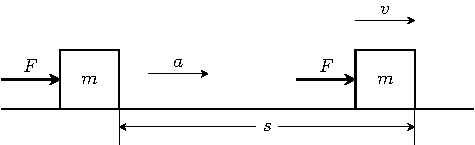
\includegraphics{fig/A/7-6.pdf}
    \caption{}\label{fig_A_7-6}
\end{figure}

设一个原来静止的物体,质量为$m$.
由于物体是静止的,没有运动,也就是没有动能,或者说动能为零.
在恒定的外力$F$作用下,物体发生一段位移$s$,得到速度$v$(图~\ref{fig_A_7-6}),获得一定的动能.设外力方向与运动方向相同,外力对物体所做的功$W=Fs$.根据牛顿第二定律,$F=ma$;根据运动学公式$v^2=2as$得到$s=v^2/2a$.将$F$和$s$的表达式代入$W=Fs$中得到
\[W=Fs=ma\times \frac{v^2}{2a}=\frac{1}{2}mv^2 \]

我们看到,外力对物体所做的功等于$\dfrac{1}{2}mv^2$这样一个跟
物体的质量和速度都有关的物理量,在物理学里就用$\dfrac{1}{2}mv^2$
这个物理量来表示物体的\NoteBold{动能}.
如果用$E_K$表示动能,那么	
\[E_K=\frac{1}{2}mv^2 \]
这就是说,\NoteUnderWave{物体的动能等于它的质量跟它的速度平方的乘积的一半}.

动能和功一样,也是标量.动能的单位跟功的单位相同,
在国际单位制里都是焦耳.
这是因为
\[1\; [{\rm kg}\cdot {\rm m^2}/{\rm s^2}]=1 \; [{\rm kg}\cdot \UmsqA ][\UmA]=1\UNm=1\UJ \]


\subsection*{练习三}
\begin{enumerate}
    \item 1976年3月8日在吉林市降落一场陨石雨,其中最大的一号陨石的质量是1770千克,假设它以45$\Ums$的速度撞击地球,计算它触地时的动能.
    \item 我国第一颗人造地球卫星的质量是173千克,速度为7.2$\Ukms$,它的动能是多少?
    \item 一个电子以$8.00\times 10^6\Ums$的速度运动.质子必须运动得多快,才能使它具有跟电子一样的动能?已知质子的质量是电子的1800倍.
    \item 有甲、乙两个物体,除了下列每一种不同点而外,这两个物体的其他情况都相同.试比较下列每一种情况下它们的动能:
    \begin{enumerate}
        \item 物体甲的速度是物体乙的两倍.
        \item 物体甲向北运动,物体乙向南运动.
        \item 物体甲做直线运动,物体乙做曲线运动.
        \item 物体甲的质量是物体乙的一半.
    \end{enumerate}
\end{enumerate}

\section{动能定理}

现在我们来进一步证明,如果物体原来就是运动的,已经具有一定的动能,受到外力推动而做加速运动,速度变大,动能增加,这时外力对物体做的功将等于物体动能的增加.

设一个质量为$m$的物体,原来的速度是$v_1$,动能是$\dfrac{1}{2}mv^2_1$,在恒定的外力$F$作用下,发生一段位移$s$,速度增加到$v_2$,动能增加到$\dfrac{1}{2}mv^2_2$.设外力方向与运动方向相同,外力$F$对物体所做的功$W=Fs$.根据牛顿第二定律,$F=ma$;根据运动学公式$v^2_2-v^2_1=2as$得到$s=(v^2_2-v^2_1)/2a$.
所以
\[Fs=ma\times \frac{v^2_2-v^2_1}{2a}=\frac{1}{2}mv^2_2-\frac{1}{2}mv^2_1 \]
或
\[W=E_{K2}-E_{K1}\]

可见,\NoteUnderWave{外力对物体所做的功的确等于物体动能的增加}.

上面我们设外力方向与运动方向相同,导出了关系式$W=E_{K2}-E_{K1}$.这个结论对外力方向与运动方向相反的情形同样适用.在这种情形下,外力所做的功是负值,而物体的运动速度减小,动能的增加也是负值.我们知道,外力对物体做负功,往往说成物体克服这个力做了功.因此,对这种情形,也可以说物体克服阻力所做的功等于动能的减少.例如在粗糙平面上运动的小车,在滑动摩擦力的作用下速度减小,这时动能的减少就等于它克服摩擦力所的功.	
	
上述结论是假定物体只受一个力而推导出来的;如物体不只受到一个力,而是受到几个力,上述结论仍旧正确.只是外力所做的功是指各个力所做的功的代数和,即外力所做的总功.这样,我们得到结论:\NoteBold{外力对物体所做的总功等于物体动能的增加}.这个结论叫做\NoteBold{动能定理}.

动能定理是力学中一条重要规律,经常用来解决有关的力学问题.下面举一个例题来说明.


\begin{example}
    一架喷气式飞机的质量为$5.0\times 10^3$千克,受到的推力为$1.8\times 10^4$牛,受到的阻力是它的重量的0.020倍,起飞速度为60$\Ums$.
    求起飞时滑跑的距离.
\end{example}


\begin{solution}
    飞机在水平方向受到的外力是推力$F$和阻力$f$,在外力作用下飞机在跑道上滑跑一段距离$s$,速度达到起飞速度$v$.飞机原来是静止的,$E_{K1}=0$,而$E_{K2}=\dfrac{1}{2}mv^2$.阻力
    $$f=0.020\times 5.0\times 10^{3}\times 9.8 \UN =9.8\times 10^2 \UN $$
    根据动能定理得到
	\[Fs-fs=\frac{1}{2}mv^2 \]
    所以
    \[\begin{split}
        s&=\frac{mv^2}{2(F-f)}\\
&=\frac{5.0\times 10^{3}\times 60^2}{2\times (1.8\times 10^{4}-9.8\times 10^2)} \Um \\
&=5.3\times 10^{2} \Um
    \end{split}\]
	\end{solution}

    这个例题也可以应用牛顿第二定律和运动学公式来解,请同学们自己做一下.动能定理的公式是在牛顿运动定律和运动学公式的基础上推导出来的,所以同一个题目用这两种方法来解,求得的结果是相同的.由于动能定理不涉及物体
    运动过程中的加速度和时间,因此应用它来解题往往比较方便.

    从例题可以看出,在利用动能定理来解力学问题的时候,先要分析物体的受力情况,并据此列出各个力所做的功,然后即可利用动能定理来求解.
    
    \subsection*{练习四}
    \begin{enumerate}
        \item 使一个物体的速度从零增加$v$,再从$v$增加到$2v$.哪种情况下做的功要多些?为什么?
        \item 在光滑平面上的物体受到沿着平面的两个力$F_1$和
        $F_2$的作用(图~\ref{fig_A_7-7}).在下列情况下,从静止开始移动2米时,物体获得的动能各是多大?
        \begin{enumerate}
            \item $F_1=10$牛,$F_2=0$;
            \item $F_1=0$,$F_2=10$牛;
            \item $F_1=F_2=5$牛.
        \end{enumerate}

\begin{figure}[htbp]
    \centering
    \begin{minipage}[t]{0.48\textwidth}
        \centering
        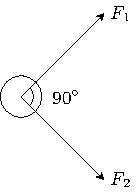
\includegraphics{fig/A/7-7.pdf}
        \caption{}\label{fig_A_7-7}
    \end{minipage}
    \begin{minipage}[t]{0.48\textwidth}
        \centering
        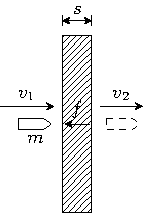
\includegraphics{fig/A/7-8.pdf}
        \caption{}\label{fig_A_7-8}
    \end{minipage}
\end{figure}



    \item 一个30牛的力水平地作用在2.0千克的物体上,使它在无摩擦的水平面上移动了3.0米的距离.然后,这个力变到15牛,又使物体移动了2.0米.物体增加的动能总共是多少?
\item 质量是2.0克的子弹,以300$\Ums$的速度水平射入厚度是10毫米的钢板(图~\ref{fig_A_7-8}),射穿后的速度是100$\Ums$.子弹受到的平均阻力是多大?

\item 一架新型喷气式战斗机的质量是$1.50\times 10^4$千克,发动机的推力是$1.11\times 10^5$牛,起飞速度是88.0$\Ums$,滑跑距离是671米.计算飞机起飞时受到的平均阻力.
    \end{enumerate}

   \section{重力势能}

   \subsection{重力势能}
   
   动能是和物体运动相联系的,静止的物体没有动能,但不能说它没有能量.除了动能,我们在初中还学过势能.举到高处的重锤具有能量,一旦让它从高处下落,就能够做功.
   拦河筑坝把水位提高,高处的水下落也能够做功(如水力发电).
   \NoteUnderWave{物体由于被举高而具有的能叫做重力势能}.举到高处的重锤、储存在高处的水都具有重力势能.

    物体由于被举高才具有重力势能,而物体在举高过程中总是要克服重力做功的.因此,重力势能跟克服重力做功有密切关系.那么,一个质量为$m$的物体,在被举到高度为$h$的
    地方,具有的重力势能是多大呢?

\begin{figure}[htbp]
    \centering
    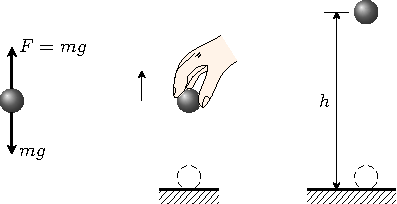
\includegraphics{fig/A/7-9.pdf}
    \caption{}\label{fig_A_7-9}
\end{figure}

    我们设想用一个与重力$mg$
    大小相等方向相反的外力$F$把物体举到高处(图~\ref{fig_A_7-9}).因为物体是在相互平衡的力作用下被举高的,物体的速度没有变化,所以它的动能也没有变化.我们知道,
物体被举高了,它的重力势能要增加,在这个过程中,我们克服重力做了功.克服重力做了多少功,重力势能就增加了多少.把物体举到高度为$h$的地方,克服重力所做的功$W=Fh=mgh$.在物理学里就用$mgh$这个物理量来表示物体的\NoteBold{重力势能}.如果用$E_P$表示重力势能,那么
\[E_P =mgh\]
这就是说,\NoteUnderWave{物体的重力势能等于它的重量和高度的乘积,惑者说,等于物体的质量、重力加速度、高度三者的乘积}.物体的质量越大,高度越大,它的重力势能就越大.

重力势能也是标量.它的单位也和功的单位相同,在国际单位制中都是焦耳.

\subsection{重力做功与重力势能的变化}

前面讲了,克服重力做了多少功,重力势能就增加多少.例如物体上升,高度增大了,这个过程中克服重力做了功,重力势能就增加了.质量为$m$的物体从高度为$h_1$的地方上升到高度为$h_2$的地方,克服重力做的功是$mg(h_2-h_1)$,重力势能则由$mgh_1$增加到$mgh_2$.反过来,如果重力对物体做了功,重力势能就要减少.
例如物体下落,高度减小了,这个过程中重力对物体做了功,重力势能就减少了.质量为$m$的物体从高度为$h_1$的地方降落到高度为$h_2$的地方,重力做的功是$mg(h_1-h_2)$,重力势能则由$mgh_1$减少到$mgh_2$.所以,在物体下落过程中,重力做了多少功,物体的重力势能就减少多少.

\subsection{重力势能的相对性}

我们知道,高度$h$是相对的.我们说某点的高度$h$为若干,这总是相对于一个水平面来说的,这个水平面的高度取作零.
例如说珠穆朗玛峰的高度是海拔8848米,这是相对于海平面来说的,海平面的高度取作零.说高山上一座建筑物的高度是5米,那是相对于高山上的一块平地说的,这块平地的高度取作零.
测量这座建筑物的高度无需再把海平面的高度取作零.和高度$h$一样,重力势能$mgh$也是相对的.我们说物体具有重力势能$mgh$,这总是相对于某一个水平面来说的,这个水平面的高度取作零,重力势能也是零.这个水平面叫做参考平面,通常选择地面作为参考平面.实际上,选择哪一个水平面作为参考平面,可视研究问题的方便而定.例如研究物体沿斜面的运动,选择通过斜面下端的水平面作为参考平面就比较方便.选择不同的参考平面,物体重力势能的数值是不同的,但这并不影响我们研究问题.我们研究有关重力势能的问题,有确定意义的总是重力势能的差值,而这个差值并不因选择不同的参考平面而有所不同.
对选定的参考平面而言,在参考平面上方的物体,高度是正值,重力势能也是正值;在参考平面下方的物体,高度是负值,重力势能也是负值.
例如取实验桌的表面作为参考平面(图~\ref{fig_A_7-10}),在斜面顶端的物体具有正的重力势能$mgh_1$,在地面上的物体具有负的重力势能$-mgh_2$.说物体具有负的重力势能,只是表示物体在该位置所具有的重力势能比它在参考平面上具有的重力势能要少,这跟用正负温度来表示温度的高低是一样的.关于负的势能我们在今后的学习中将会
碰到.
\begin{figure}[htbp]
    \centering
    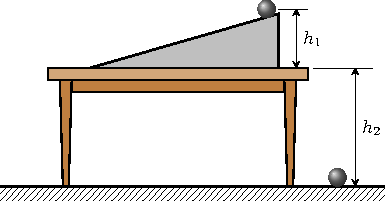
\includegraphics{fig/A/7-10.pdf}
    \caption{正重力势能和负重力势能}\label{fig_A_7-10}
\end{figure}

\section{重力做功的特点和重力势能}
上一节我们讲到了克服重力做了多少功,重力势能就增加了多少;重力对物体做了多少功,重力势能就减少了多少.这个问题还有进一步讨论的必要.为此我们要先研究一下重力做功的特点.

\subsection{重力做功的特点}
\begin{figure}[htbp]
    \centering
    \begin{minipage}[b]{0.48\linewidth}
    	\centering
    	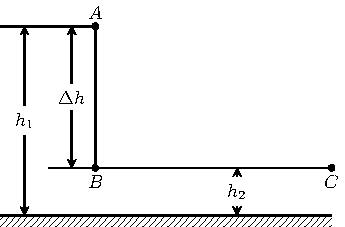
\includegraphics{fig/A/7-11.pdf}
    	\caption{}\label{fig_A_7-11}
    \end{minipage}
    \begin{minipage}[b]{0.48\linewidth}
    	\centering
    	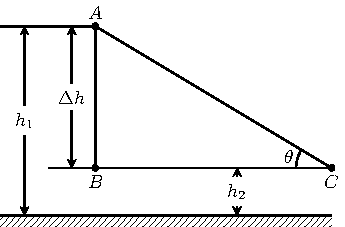
\includegraphics{fig/A/7-12.pdf}
    	\caption{}\label{fig_A_7-12}
    \end{minipage}
\end{figure}

设一个质量是$m$的物体,从原来高度
是$h_1$的$A$点自由下落到高度是$h_2$的$B$点再水平移到$C$点(图~\ref{fig_A_7-11}),由于物体水平移动中重力并不做功,所以在整个过程中重力对物体所做的功就等于物体由$A$点自由下落到$B$点中重力所做的功:
\[W_G=mg\Delta h=mgh_1-mgh_2\]
如果让这个物体沿着斜面滑下(图~\ref{fig_A_7-12}),从原来高度是$h_1$的$A$点滑到高度是$h_2$的$C$点,物体沿斜面滑下的距离是$s$,重力所做的功是
\[W_G=mg\sin\theta \cdot s=mg\Delta h=mgh_1-mgh_2\]




现在我们来看这个物体沿着任一路径$AB$从原来高度是$h_1$的$A$点运动到高度是$h_2$的$B$点,重力所做的功是多少(图~\ref{fig_A_7-13}).
我们把路径$AB$分成许多很短的间隔$AA_1 $,$ A_1A_2 $,$ A_2A_3 $,$ \cdots$,使每个间隔都相当于一个斜面.
设每个小斜面的高度是$\Delta h_1 $,$ \Delta h_2 $,$ \Delta h_3 $,$ \cdots$,那么物体通过每个小斜面时重力所做的功是$mg\Delta h_1 $,$ mg\Delta h_2 $,$ mg\Delta h_3 $,$ \cdots$.
物体通过路径$AB$时重力所做的功等于重力在每个小斜面上所做的功的代数和,即
\[\begin{split}
W_G&= mg\Delta h_1+mg\Delta h_2+mg\Delta h_3+\cdots\\
&=mg\Delta h\\
&=mgh_1-mgh_2
\end{split} \]


\begin{figure}[htbp]
	\centering
	\begin{minipage}[t]{0.55\linewidth}
		\centering
		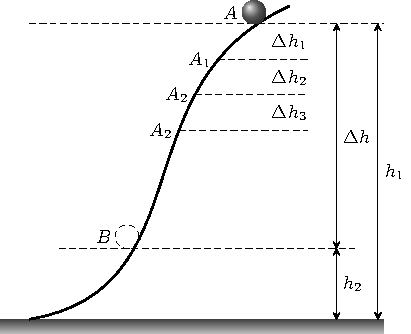
\includegraphics{fig/A/7-13.pdf}
		\caption{}\label{fig_A_7-13}
	\end{minipage}
	\hfil
	\begin{minipage}[t]{0.35\linewidth}
		\centering
		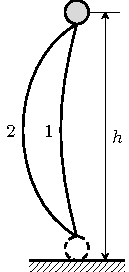
\includegraphics{fig/A/7-14.pdf}
		\caption{}\label{fig_A_7-14}
	\end{minipage}
\end{figure}

我们看到,\NoteUnderWave{重力对物体所做的功只跟起点$A$和终点$B$的位置有关,而跟物体运动的路径无关.也就是说,只要起点和终点的位置相同,不论物体沿着什么路径运动,重力所做的功都相同}.

这就是重力做功的特点.并不是任何力做功都有这个特点.摩擦力做功就没有这个特点.

\subsection{重力势能的进一步讨论}



重力做功的上述特点对于物理学里能够引入重力势能是有决定意义的.原来,如果重力做功没有这个特点,而是与路径有关,那么,我们分别沿着不同的路径把一个物体由地面举到高度为$h$的一点(图~\ref{fig_A_7-14}),克服重力所做的功将不相同.
设沿着路径1把物体举高时克服重力所做的功是$W_1$,沿着路径2把物体举高时克服重力所做的功是$W_2$.这样,位于高度$h$上的物体的重力势能到底等于$W_1$还是等于$W_2$呢?这个重力势能也就没有意义了!可见,正是由于重力做功与路径无关,重力势能的改变才有确定值,在物理学中才可以引入重力势能这个概念.


克服摩擦力做的功是与路径有关的.物体沿不同路径从一个位置移到另一位置,克服摩擦力做的功一般是不相等的.
因此,在物理学中就不存在“摩擦势能”这个概念.


\subsection{势能属于系统} 

重力势能的改变是由重力做功来确定的,而重力是地球和物体之间的相互作用力,重力做功涉及的是重力这种相互作用力以及地球和物体的相对位置,所以严格说来,重力势能是地球和物体共有的,而不是物体单独具有的.在物理学中通常把相互作用的物体的全体叫做\NoteBold{系统}.
重力势能是属于地球和物体所组成的这个系统的.
通常所说的物体具有多少重力势能,只能理解为一种简略的说法.

除了重力势能,还有其他形式的势能.
势能是系统由于其中各物体之间存在相互作用而具有的能,而且是由各物体的相对位置决定的.例如分子之间由于存在相互作用而具有由分子间相对位置决定的势能,叫做分子势能.电荷之间由于存在相互作用而具有由电荷间相对位置决定的势能,叫做电
势能.分子势能或电势能分别属于分子或电荷所组成的系统,也不是一个分子或一个电荷单独具有的.

\subsection*{练习五}
下列各题中都以地面作参考平面.
\begin{enumerate}
    \item 体积相同的铝球和铅球,处在同一高度的地方,哪一
    个的重力势能较大?
    \item 质量是2千克的物体位于0.8米高的桌面上,这个物体具有多少重力势能?
    \item 图~\ref{fig_A_7-15} 是几个斜面,它们的高度相同,而倾角不同.
    让质量相同的物体沿斜面从顶端运动到底端.
    试根据功的公式来计算沿不同斜面重力所做的功,证明这个功跟斜面的倾角无关.
\begin{figure}[htbp]
    \centering
    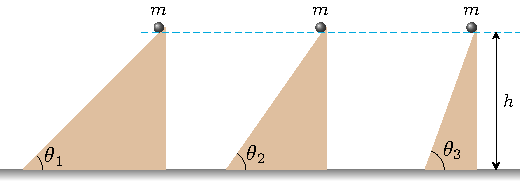
\includegraphics{fig/A/7-15.pdf}
    \caption{}\label{fig_A_7-15}
\end{figure}
\item 图~\ref{fig_A_7-16} 表示一个斜抛物体的运动,当物体由抛出位置1运动到最高位置2时,重力所做的功是多少?物体克服重力所做的功是多少?由位置2运动到跟位置1在同一水平面上的位置3时,重力所做的功是多少?由位置1运动到位置3时,重力所做的功是多少?
\end{enumerate}

\begin{figure}[htbp]
    \centering
    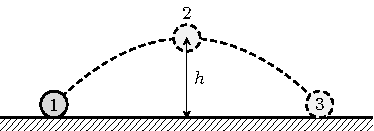
\includegraphics{fig/A/7-16.pdf}
    \caption{}\label{fig_A_7-16}
\end{figure}


\section{弹性势能}
这一节我们研究物体因发生弹性形变而具有的势能,这种势能叫做\NoteBold{弹性势能}.物体发生弹性形变的时候,物体的各个部分之间发生弹力的相互作用.正像地球和物体之间由于有重力的相互作用,因而地球和物体组成的系统具有重力势能一样,发生弹性形变的物体的各个部分之间由于有弹力的相互作用,因而由这些部分组成的系统,亦即发生弹性形变的物体本身,就具有弹性势能.

任何发生了弹性形变的物体都具有弹性势能.卷紧了的
发条,拉长或压缩了的弹簧,拉弯了的弓,正在击球的网球拍或羽毛球拍,正在支撑运动员上跳的撑竿等等,都具有弹性势能(图~\ref{fig_A_7-17}).
\begin{figure}[htbp]
    \centering
    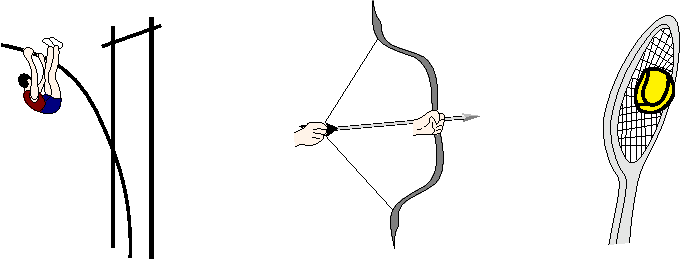
\includegraphics{fig/A/7-17.pdf}
    \caption{任何发生弹性形变的物体都具有弹性势能}\label{fig_A_7-17}
\end{figure}

弹性势能和弹力做功密切相关,它们的关系类似于重力势能和重力做功的关系.
下面以弹簧为例定性地加以说明.


用外力压缩或伸长弹簧的时候(图~\ref{fig_A_7-18}),外力要克服弹
力做功,克服弹力做多少功,弹簧的弹性势能就增加多少.
把被压缩或伸长的弹簧放开的时候(图~\ref{fig_A_7-19}),弹力可以推动其他物体做功,弹力做多少功,弹簧的弹性势能就减少多少.

\begin{figure}[htbp]
	\centering
	\begin{minipage}[t]{0.46\linewidth}
		\centering
		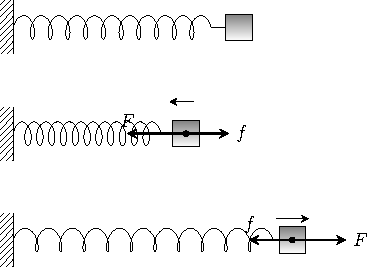
\includegraphics{fig/A/7-18.pdf}
		\caption{克服弹力做功,弹簧的弹性势能增加。图中$F$表示外力,$f$表示弹力。上图是没有发生形变的弹簧.}\label{fig_A_7-18}
	\end{minipage}
	\hfill
	\begin{minipage}[t]{0.42\linewidth}
		\centering
		\centering
		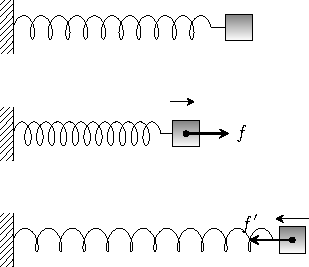
\includegraphics{fig/A/7-19.pdf}
		\caption{弹力做功,弹簧的弹性势能减少.图中$f$表示弹力。上图是没有发生形变的弹簧.}\label{fig_A_7-19}
	\end{minipage}
\end{figure}

弹簧的弹性势能跟弹簧被压缩或拉伸的长度有关系.一
个没有被压缩或拉伸的弹簧,弹性势能为零.
弹簧被压缩或拉伸的时候,它被压缩或拉伸得越大,克服弹力所做的功越多,弹簧的弹性势能就越大.另外,弹簧的弹性势能还跟弹簧的劲度系数有关系.不同的弹簧被压缩或拉伸相同的长度,劲度系数越大,克服弹力做的功越多,因而弹簧的弹性势能就越大.

\section{机械能守恒定律}
\subsection{机械能的相互转化}

动能和势能(重力势能和弹性势能)统称为\NoteBold{机械能}.一种形式的机械能是可以和另一种形式的机械能相互转化的,下面我们看一些例子.

物体自由下落或者沿着光滑斜面滑下的时候,重力对物
体做功,物体的重力势能减少.
而物体的速度越来越大,表示物体的动能增加了.这时重力势能转化成动能.

原来具有一定速度的物体,在竖直上升或者沿着光滑斜面上升的时候,物体克服重力做功,速度越来越小,物体的动能减少了,同时物体的高度增加,重力势能增加了.这时动能转化成重力势能.

弹性势能也可以跟动能相互转化.放开一个被压缩的弹簧,它可以把一个跟它接触的小球弹出去.这时弹力做功,弹簧的弹性势能减少,同时小球得到一定的速度,动能增加.放开被拉开的弓把箭射出去,这时弓的弹性势能减少,箭的动能增加.

从这些例子我们看到,机械能的相互转化是通过重力或弹力做功来实现的.重力或弹力做功的过程,也就是机械能从一种形式转化成另一种形式的过程.下面我们进一步来研究
重力或弹力做功的多少跟这种转化的定量关系.
	
\subsection{机械能的守恒} 
\begin{figure}[htbp]
    \centering
    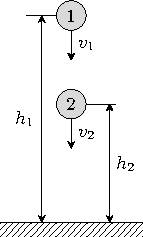
\includegraphics{fig/A/7-20.pdf}
    \caption{}\label{fig_A_7-20}
\end{figure}

我们先用自由落体作例子定量的研究动能和重力势能的转化(图~\ref{fig_A_7-20}).设有一个质量是$m$的物体,从高度是$h_1$的地方(起点)下落到高度是$h_2$的地方(终点).设
物体在起点的速度为$v_1$,在终点的速度为$v_2$.物体在下落过程中,重力做了功,从动能定理知道,重力所做的功等于物体动能的增加,即
\[W_G=\frac{1}{2}mv_2^2-\frac{1}{2}mv^2_1 \]
另一方面,从重力做功与重力势能的关系知道,重力所做的功等于重力势能的减少,即
\[W_G=mgh_1-mgh_2\]
这样,我们得到
\[\frac{1}{2}mv_2^2-\frac{1}{2}mv^2_1 =mgh_1-mgh_2\]
这就是说,重力做了多少功,就有多少重力势能转化成等量的动能.把上式移项后得到
\[ \frac{1}{2}mv^2_2 +mgh_2=\frac{1}{2}mv^2_1 +mgh_1\]
上式表示,物体在自由下落中,它的重力势能转化成动能,但在任何时刻,动能和重力势能之和亦即它的机械能保持不变.

上述结论不仅对自由落体是正确的,可以证明,在只有重力做功的情形下,它总是正确的.所谓只有重力做功,是指:物体只受重力,不受其他的力,如自由落体和各种抛体运动的情形;或者除重力而外还受其他的力,但其他力并不做功,物体沿光滑斜面运动就属于这种情形.

\NoteBold{在只有重力做功的情形下,物体的动能和重力势能发生相互转化,但总的机械能保持不变}.这个结论叫做\NoteBold{机械能守恒定律},它是力学中一条重要规律,又是更普遍的能的转化和
守恒定律的一个特例.

不但动能和重力势能的相互转化中机械能保持不变,在弹性势能和动能的相互转化中,如果只有弹力做功,机械能也是保持不变的.

\subsection*{练习六}
\begin{enumerate}
    \item 在下面列举的各个实例中,除 (\ref{exe_A_7-6-1.1}) 外都不计空气阻力,哪些机械能是守恒的?说明理由.
    \begin{enumerate}
        \item \label{exe_A_7-6-1.1} 跳伞员带着张开的降落伞在空气中匀速下落.
        \item 抛出的手榴弹或标枪做斜抛运动.
        \item 用细绳拴着一个小球,绳的一端固定,使小球在光滑的水平面上做匀速圆周运动.
        \item 用细绳拴着一个小球,绳的一端固定,使小球在竖直平面上做圆周运动.
        \item 物体沿着光滑的曲面滑下(图~\ref{fig_A_7-21a}).
        \item 拉着一个物体沿着光滑的斜面匀速上升(图~\ref{fig_A_7-21b}).
        \item 在光滑水平面上运动的小球,碰到弹簧上,把弹簧压缩后又被弹簧弹回来(图~\ref{fig_A_7-21c}).
    \end{enumerate}
\begin{figure}[htbp]
    \centering
    \begin{subfigure} {0.3\linewidth} 
        \centering
        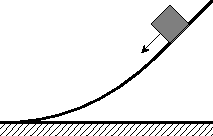
\includegraphics{fig/A/7-21a.pdf} 
        \caption{}\label{fig_A_7-21a} 
    \end{subfigure}
    \hfil
    \begin{subfigure} {0.3\linewidth} 
        \centering
        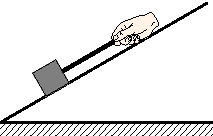
\includegraphics{fig/A/7-21b.pdf}
        \caption{}\label{fig_A_7-21b} 
    \end{subfigure}
    \hfil
    \begin{subfigure} {0.3\linewidth} 
        \centering
        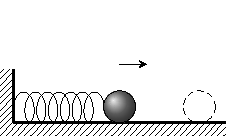
\includegraphics{fig/A/7-21c.pdf}
        \caption{}\label{fig_A_7-21c} 
    \end{subfigure}
    \caption{}\label{fig_A_7-21}
\end{figure}

    \item  做下面的实验,把物体拴在细线上悬挂起来,做成
    一个单摆(图~\ref{fig_A_7-22}).把物体从平衡位置$O$拉到$B$,放手后观察物体的来回摆动,把铅笔放在位置1和2,可以看到物体仍然要升到跟$B$同样高的$C_1$和$C_2$.解释这个现象.
\begin{figure}[htbp]
    \centering
    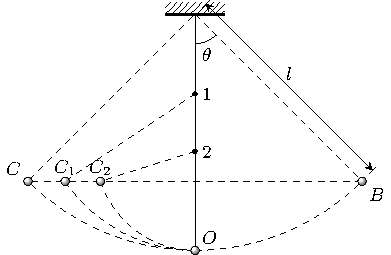
\includegraphics{fig/A/7-22.pdf}
    \caption{}\label{fig_A_7-22}
\end{figure}
\end{enumerate}

\section{机械能守恒定律的应用}

机械能守恒定律广泛用来解决各种力学问题,下面通过例题来说明它的应用.


\begin{example}
    竖直上抛的物体,初速度是$v_0$,求物体上升的最大高度.不计空气阻力.
\end{example}


\begin{solution}
    这个问题我们在第\ref{chapter-rectilinear-motion}章已经研究过:现在用机械能守恒
定律来处理.竖直上抛的物体只受重力的作用,因而机械能守恒.

物体抛出时,动能是$\dfrac{1}{2}mv^2_0$ ,重力势能为零,机械能$E_1=\dfrac{1}{2}mv^2_0$.物体达到最大高度$H$时,动能为零,重力势能是$mgH$,机械能$E_2=mgH$.因为$E_1=E_2$,所以
\[\begin{split}
    mgH&=\dfrac{1}{2}mv^2_0\\
    H&=\frac{v^2_0}{2g}
\end{split}\]
\end{solution}

我们看到,用机械能守恒定律求得的答案跟我们在第\ref{chapter-rectilinear-motion}章用运动学的方法求得的结果完全相同.

用机械能守恒定律不但能处理直线运动问题,而且能处理曲线运动问题.直接应用牛顿第二定律和运动学的知识来处理力学问题特别是曲线运动,固然可以确定运动物体在任一时刻的位置和速度,从而获得关于这个力学问题的全面知
识,但往往需要用高等数学来计算,有的计算还相当复杂.
用机械能守恒定律来处理,却可以相当简便.


\begin{example}
    一个摆长是$\ell$的单摆,最大偏角是$\theta$,求单摆在最低位置的速度(图~\ref{fig_A_7-22}).
\end{example}


\begin{solution}
    这个问题直接用牛顿第二定律和运动学的知识来处理,就需要用高等数学.
    现在用机械能守恒定律来处理.

摆锤受到两个力:重力和悬线的拉力.悬线的拉力始终垂直于摆锤的运动方向,不做功,所以单摆的机械能守恒.

选择摆锤在最低点时所在的水平面作参考平面.
摆锤在最高点时,动能为零,重力势能是$mg(\ell-\ell\cos\theta)$,机械能$E_1=mg(\ell-\ell\cos\theta)$. 摆锤在最低点时,动能是$\dfrac{1}{2}mv^2$,重力势能
为零,机械能$E_2=\dfrac{1}{2}mv^2$.因为$E_1=E_2$,所以
\[\begin{split}
    \dfrac{1}{2}mv^2&=mg(\ell-\ell\cos\theta)\\
    v&=\sqrt{2g\ell(1-\cos\theta)}
\end{split}\]
\end{solution}

我们看到,由于机械能守恒定律只涉及开始状态和终了状态的机械能,不涉及中间运动过程的细节,因此用它来处理问题相当简便.

当然,有的问题只用机械能守恒定律还不能完全解决.例如要想求单摆在最低位置时悬线的拉力$F$,就还需要应用圆周运动的知识.
应用机械能守恒定律求出速度$v$之后,我们不难求出悬线的拉力:
\[F=mg+\frac{mv^2}{\ell}=mg-2mg (1-\cos\theta)\]

解决力学问题,先从能量的观点入手分析,往往带来方便.
应用机械能守恒定律来解决力学问题,也要先分析物体的受力情况.在动能和重力势能的相互转化中,如果只有重力做功,其他力不做功,就可以应用机械能守恒定律.

守恒定律不仅给处理问题带来方便,而且有更深刻的意义.物理世界是千变万化的,但是人们发现有些物理量在一定条件下是守恒的,可以用这些“守恒量”来表示物理世界变化的规律,这就是守恒定律.机械能守恒定律就是其中一个.
正因为自然界存在着“守恒量”,而且某些守恒定律的适用范围很广泛,所以在物理学中寻求“守恒量”已经成为物理研究工作的一个重要方面.
下一章我们将学习另一个守恒定律——动量守恒定律.

\subsection*{练习七}
\begin{enumerate}
    \item 滑雪运动员从25米高的山坡上滑下,如果阻力忽略不计,他滑到坡底时的速度是多大?
    \item 物体从高的光滑斜面的顶端滑下,证明物体到达斜面末端时的速度 $v=\sqrt{2gH}$.
    \item 蒸汽打桩机的重锤的质量是250千克,把它提升到离地面25米高处,然后让它自由落下.计算:
    \begin{enumerate}
        \item 重锤在最高点的动能、重力势能和机械能.
        \item 重锤下落10米时的重力势能、动能和速度.
        \item 重锤落到地面时的重力势能、动能和速度.
    \end{enumerate}
\item 要使一球着地后回跳的高度超过原高10米,必须以多大速度将它下抛?不计球击地时的能量损失.
\item 一个物体从距地面40米的高处自由落下,经过几秒后,该物体的动能和重力势能相等?$g=10\Umsq$.
\end{enumerate}

\section{功和能}\label{sec-A-07-work-and-energy}
前面我们研究了机械能的守恒,但是我们经常可以看到机械能并不守恒的事例.仔细考察这类事例可以发现,如果除了重力还有其他力对物体做功,物体的动能和重力势能之和,即物体的机械能,就发生变化.

火车在水平的轨道上开出,重力势能没有变化,动能越来越大,机械能在不断增加.火车机械能的增加是因为牵引力对它做了功,牵引力做多少功,火车的机械能就增加多少.

起重机加速提升重物,重物的动能和重力势能都越来越大,机械能在不断增加.重物机械能的增加是因为钢索的拉力对它做了功,拉力做多少功,重物的机械能就增加多少.

跳伞员在张开降落伞后匀速下降,动能没有变化,重力势
能越来越小,他的机械能在不断减少.跳伞员机械能的减少是因为他克服空气阻力做了功.克服空气阻力做了多少功,机械能就减少多少.

子弹射入墙壁,最后停在墙里,子弹的机械能减少.子弹机械能的减少是因为它克服摩擦力做了功.克服摩擦力做了多少功,机械能就减少多少.

总之,\NoteUnderWave{物体的机械能发生变化,都是因为其他力对物体做了功;其他力做多少功,机械能就增加多少,克服其他力做多少功,机械能就减少多少}.

增加了的机械能并不是凭空产生的.飞机、火车、汽车开动的时候,发动机的牵引力做功,它们的机械能增加了,同时也消耗了燃料中储存的化学能.牵引力做功的过程,就是化学能转化成机械能的过程.
牵引力做多少功,就有多少化学能转化成机械能.

减少的机械能也不能无影无踪地消失.子弹射入墙壁的时候,克服摩擦力做功,它的机械能减少,同时产生了热能,使子弹和墙壁的温度升高.克服摩擦力做功的过程,就是机械能转化成热能的过程.克服摩擦力做多少功,就有多少机械能转化成热能.

能量既不能凭空产生,也不能无影无踪地消失,不同形式的能在相互转化中保持守恒.做功的过程就是能从一种形式转化成另一种形式的过程.在机械能不守恒的运动中,做了多少功,就有多少机械能和其他形式的能发生转化.\NoteUnderWave{功是能的转化的量度}.

\section*{复习题}
\begin{enumerate}
    \item 做功的两个不可缺少的因素是什么?计算功的公式是什么?
    \item 什么叫功率?写出计算功率的公式.
    \item 什么叫动能?定义动能的公式是什么?
    \item 动能定理的内容是什么?写出它的公式.
    \item 什么叫重力势能?定义重力势能的公式是什么?
    \item 重力做功有什么特点?这个特点在引入重力势能上有什么意义?
    \item 什么叫弹性势能?什么叫机械能?
    \item 机械能守恒定律的内容是什么?在什么条件下机械能守恒?
    \item 从能量的观点来分析和处理力学问题有什么好处?谈谈你自己的体会.
    \item 这一章的内容较多,你能不能抓住一个基本思路把这一章的知识联系起来?如果你还做不到这一点,建议你认真地再读一读第\ref{sec-A-07-energy}节能量和第\ref{sec-A-07-work-and-energy}节功和能这两节的课文.
\end{enumerate}

\section*{习题}
\begin{enumerate}
    \item 一个原来静止的物体,在力$F$的作用下,沿着力的方向移动一段距离$s$,得到速度$v$.如果移动的距离不变,力$F$增大到$n$倍,得到的速度也增大到$n$倍.这话对吗?速度应该增大到多少倍?
    \item 在水平面上有两个质量不同而具有相同动能的物
体,它们所受的阻力相等.这两个物体停止前经过的距离是否相同?停下来所用的时间是否相同?
\item 质量是$m$千克的物体自由落下,在第1秒内和第2秒内物体重力势能的减少各是多少?
\item 从地面竖直上抛一个物体,质量是0.2千克,经过8秒落回原地.物体抛出时的动能是多少?从被抛出到最高点,物体克服重力所做的功是多少?物体上升到最高点时的重力势能是多少?不计空气阻力.
\item 一个人站在10米高的楼上沿斜上方抛出一个小球,初速度的大小是10$\Ums$,抛出角是30$^\circ$,小球落地时速度是多大?如果初速度的大小不变,沿斜下方抛出小球,抛射角是45$^\circ$,小球落地时速度是多大?用其他某个角度抛出,结果又怎
样?不计空气阻力.
\item 利用机械能守恒定律,你能算出平抛和斜抛物体通过任意位置时速度的大小吗?怎样计算?
\item 质量是0.25千克的球以2.0$\Ums$的速度向右运动,然后沿着图~\ref{fig_A_7-23} 所示的光滑的凹面滚动,这个小球在凹面的右侧能滚上多高?如果在$P$点把球从静止放开,它能滚上多高?
\begin{figure}[htbp]
    \centering
    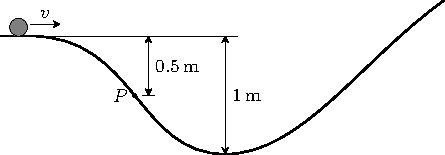
\includegraphics{fig/A/7-23.pdf}
    \caption{}\label{fig_A_7-23}
\end{figure}

\item  一颗子弹以700$\Ums$的速度打穿第一块木板后,速度减低到500$\Ums$.如果让它继续打穿第二块同样的木板,它的速度将变为多大?它能否再打穿第三块同样的木板?
\item  列车经过一段长2.1千米的平直铁路,速度从54$\Ukmh$增加到72$\Ukmh$,列车重1400吨,列车受到的阻力
是车重的$k=0.003$倍.求机车的功率.
\item  在一个农村小水电站里,上下游的水位差是3米,每秒钟有0.5$\Umc$的水流过发电机的水轮机,从水轮机流出的水的速度是3$\Ums$,上游水的流速忽略不计.设水流能的70\%可以转化成电能,求这个小水电站发出的电功率.
\item  飞机、轮船所受的空气或水的阻力并不是固定的,它跟飞机、轮船的速度有关.当速度很大时,阻力与速度的平方成正比.
试证明:这时要把飞机、轮船的最大速度增大到2倍,发动机的额定功率要增大到8倍才行.这就是在增大飞机、轮船等交通工具的速度方面,每取得一个新的成就都很不容易的原因.
\item 一辆汽车沿着平直的道路行驶,遇有紧急情况而刹车,刹车后轮子只滑动不滚动.
从刹车开始到汽车停下来,汽车前进12米.已知轮胎与路面之间的滑动摩擦系数$\mu=0.7$.求刹车前汽车的行驶速度.不计空气阻力.
\item 一辆5吨的载重汽车开上一个坡路,坡路长$s=100$米.
坡顶和坡底的高度差$h=10$米,汽车上坡前的速度是10$\Ums$,上到坡顶时减为5.0$\Ums$.汽车受到的摩擦阻力是车重的$k=0.05$倍.求汽车的牵引力.取$g=10\Umsq$.
 
讨论:在这个题目里,汽车的牵引力做多少功?汽车增加
的机械能是多少?其中动能和重力势能各是多少?克服摩擦而转化成的热能是多少?
\item 一个滑雪的人从高度为$h$的斜坡上由静止开始滑下,然后在水平面滑行一段距离停下来(图~\ref{fig_A_7-24}).已知斜面的倾角为$\theta$,滑雪板和雪之间的滑动摩擦系数为$\mu$,求滑雪人在水平面上滑行的距离$s_1$.你能不能求出滑雪人通过的水
平距离$s$?其他条件不变,只改变斜坡的倾角$\theta$,水平距离$s$是否改变?为什么?
\begin{figure}[htbp]
    \centering
    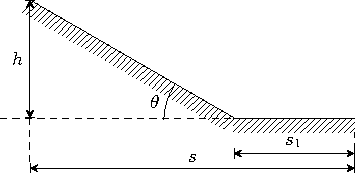
\includegraphics{fig/A/7-24.pdf}
    \caption{}\label{fig_A_7-24}
\end{figure}

\item 要使小球滑到光滑的离心轨道顶端时不落下来(图~\ref{fig_A_7-25}),至少应使它在斜轨上多高处由静止开始下滑?


\begin{figure}[htbp]
    \centering
    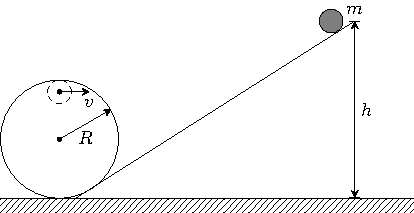
\includegraphics{fig/A/7-25.pdf}
    \caption{}\label{fig_A_7-25}
\end{figure}

\end{enumerate}




